\documentclass[aspectratio=169, 10pt]{beamer}

%Packages
\usepackage[utf8]{inputenc}
\usepackage{amsmath}
\usepackage{amsfonts}
\usepackage{amssymb}
\usepackage{listings}
\usepackage{xcolor}
\usepackage{tikz}
\usepackage{hyperref}
\usepackage{algorithm}
\usepackage{algpseudocode}

% =========================
% THEME & COLORS (Black Background)
% =========================
\definecolor{bgblack}{RGB}{0,0,0}
\definecolor{fgwhite}{RGB}{240,240,240}
\definecolor{accentcyan}{RGB}{0, 255, 255}
\definecolor{softgray}{RGB}{100,100,100}
\definecolor{codebg}{RGB}{20,20,20}
\definecolor{codegreen}{RGB}{0,200,100}
\definecolor{codeblue}{RGB}{80,160,255}
\definecolor{codepurple}{RGB}{200,100,255}

\setbeamercolor{background canvas}{bg=bgblack}
\setbeamercolor{normal text}{fg=fgwhite}
\setbeamercolor{frametitle}{fg=accentcyan}
\setbeamercolor{title}{fg=accentcyan}
\setbeamercolor{structure}{fg=accentcyan}
\setbeamercolor{item}{fg=accentcyan}
\setbeamercolor{section in toc}{fg=fgwhite}
% Make main text slightly smaller for a more compact layout
% (reduce global font a bit without changing documentclass option)
\setbeamerfont{normal text}{size=\small}
\setbeamerfont{frametitle}{size=\small}
\setbeamerfont{title}{size=\small}
\setbeamerfont{author}{size=\small}
\setbeamerfont{institute}{size=\scriptsize}

% Listings setup for LAMMPS/Python code
\lstset{
    backgroundcolor=\color{codebg},
    basicstyle=\ttfamily\footnotesize\color{fgwhite},
    commentstyle=\color{softgray},
    keywordstyle=\color{codepurple},
    numberstyle=\footnotesize\color{softgray},
    stringstyle=\color{codegreen},
    breaklines=true,
    frame=leftline,
    rulecolor=\color{accentcyan},
    numbers=left,
    xleftmargin=10pt,
}

% Title Info
\title{Solvent Structure around Nanoparticles}
\subtitle{Investigating Hydrophobicity via MD Simulations}
\author{\href{https://shuvam-banerji-seal.github.io/}{Shuvam Banerji Seal} (22MS076)}
\institute{Indian Institute of Science Education and Research Kolkata}
\date{\today}

\begin{document}

% =========================
% SLIDE 1: Title
% =========================
\begin{frame}
    % \centering
    % \Huge \textbf{\textcolor{accentcyan}{Solvent Structure around Nanoparticles}} \\
    % \vspace{0.5cm}
    % \large Tuning Hydrophobicity \& Hydrophilicity \\
    % \vspace{1cm}
    % \normalsize \textbf{Shuvam Banerji Seal} \\
    % \scriptsize \url{https://shuvam-banerji-seal.github.io/} \\
    % \vspace{0.5cm}

    \titlepage
    \scriptsize Repository: \url{git@github.com:Shuvam-Banerji-Seal/Solvent-Structure-around-NanoParticles.git}
\end{frame}

% =========================
% SLIDE 2: TOC
% =========================
\begin{frame}[allowframebreaks]{Table of Contents}
    \tableofcontents
\end{frame}

% =========================
% SECTION: Intro
% =========================
\section{Introduction \& Problem Statement}

\begin{frame}{Problem Statement}
    \begin{columns}
        \column{0.6\textwidth}
        \textbf{Core Scientific Question:}
        \begin{itemize}
            \item How does the solvent (water) reorganize itself around a nanoparticle (C60)?
            \item How does this reorganization change as we tune the interaction strength ($\epsilon_{CO}$)?
            \item \textit{Hypothesis:} The transition from hydrophobic to hydrophilic induces a structural phase transition in the solvation shell.
        \end{itemize}
        
        \vspace{0.5cm}
        \textbf{The Machine Learning Angle:}
        \begin{itemize}
            \item Can we generate descriptors (RDF fingerprints, Voronoi tessellation) from MD trajectories?
            \item Can ML models predict aggregation propensity based purely on local solvent structure?
        \end{itemize}

        \column{0.4\textwidth}
        \centering
        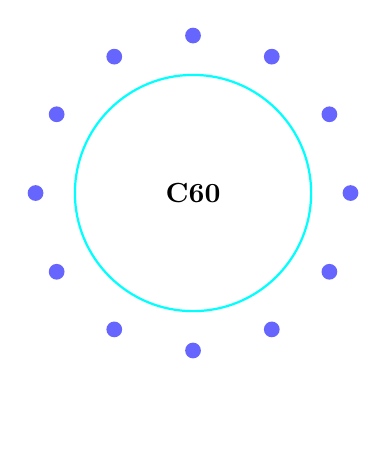
\begin{tikzpicture}
            \draw[accentcyan, thick] (0,0) circle (1.5cm);
            \node at (0,0) {\textbf{C60}};
            \foreach \angle in {0,30,...,330}
                \fill[blue!60] (\angle:2cm) circle (0.1cm);
             \node[below, white] at (0,-2.5) {Solvation Shell};
        \end{tikzpicture}
    \end{columns}
\end{frame}

% =========================
% SECTION: System Overview
% =========================
\section{System Overview}

\begin{frame}{The Simulated System}
    \textbf{Composition:}
    \begin{itemize}
        \item \textbf{Solute:} 3 $\times$ Buckminsterfullerene (C60) Molecules ($N_{atoms} = 180$).
        \item \textbf{Solvent:} $\sim$2000 Water molecules (TIP4P/2005 model).
        \item \textbf{Box:} Cubic $40 \times 40 \times 40$ \AA$^3$ (Periodic Boundary Conditions).
    \end{itemize}

    \vspace{0.5cm}
    \textbf{Physics Engine (LAMMPS):}
    \begin{itemize}
        \item \textbf{Force Field:} Lennard-Jones + Coulombic (Long Range).
        \item \textbf{Thermostat/Barostat:} Nosé-Hoover (NVT/NPT).
        \item \textbf{Constraints:} SHAKE algorithm for rigid water bonds.
    \end{itemize}
\end{frame}

% =========================
% SECTION: Methodology - Files
% =========================
\section{Methodology: System Construction}

\begin{frame}{Step 1: Raw Data (\texttt{C60.data})}
    \textbf{Origin:} 
    Derived from the standard XYZ coordinates available in the LAMMPS library.
    
    \vspace{0.5cm}
    \textbf{Content:}
    \begin{itemize}
        \item Contains spatial coordinates $(x, y, z)$ for 60 Carbon atoms.
        \item \textit{Limitation:} Purely geometric. No bonding topology (bonds, angles, dihedrals) is defined in the raw file.
    \end{itemize}
    
    \vspace{0.5cm}
    \textit{We must computationally infer the topology to treat C60 as a rigid, bonded molecule.}
\end{frame}

% =========================
% TOPOLOGY GENERATION
% =========================
\begin{frame}[fragile]{Step 2: Topology Generation (\texttt{generate\_C60\_bonded.py})}
    \textbf{Objective:} Transform point cloud to bonded graph.
    \textbf{Bond Criteria:} C-C bond length in Fullerene $\approx 1.4$ \AA. Threshold: $1.3 \le r_{ij} \le 1.5$ \AA.

    \begin{columns}
    \column{0.5\textwidth}
    \begin{algorithmic}[1]
        \State Read Atoms $A = \{a_1, ..., a_{60}\}$
        \State $Bonds \leftarrow []$
        \For{$i \in 1 \dots 60$}
            \For{$j \in (i+1) \dots 60$}
                \State $d_{ij} = \sqrt{(x_i-x_j)^2 + ...}$
                \If{$1.3 \le d_{ij} \le 1.5$}
                    \State $Bonds.append((i, j))$
                \EndIf
            \EndFor
        \EndFor
        \State \textbf{Verify:} Count bonds per atom
        \If{$\forall i, Count(i) == 3$}
            \State Write \texttt{C60\_bonded.data}
        \Else
            \State \textbf{Error:} Invalid Topology
        \EndIf
    \end{algorithmic}
    
    \column{0.5\textwidth}
    \textbf{Mathematical Basis:}
    Euclidean Distance Metric:
    \begin{equation}
        r_{ij} = ||\mathbf{r}_i - \mathbf{r}_j||_2
    \end{equation}
    Graph Theory Constraint:
    \begin{equation}
        deg(v) = 3, \quad \forall v \in V_{C60}
    \end{equation}
    Total Bonds:
    \begin{equation}
        |E| = \frac{1}{2} \sum deg(v) = \frac{60 \times 3}{2} = 90
    \end{equation}
    \end{columns}
\end{frame}

% =====================================================================
% SECTION: Detailed Script Analysis - Validation
% =====================================================================
\section{Script 1: Build \& Validate}

% --- Slide: Initialization & Potentials ---
\begin{frame}[fragile]{Validation Script: Initialization \& Force Field}
    \textbf{1. Atom Definition:}
    \begin{lstlisting}[language=bash]
    units real          # Energy: kcal/mol, Dist: Angstrom, Time: fs
    atom_style full     # Attributes: ID Mol Type Charge X Y Z
    \end{lstlisting}
    \textit{Physics:} `full` is required because TIP4P water relies on partial charges ($q_O = -1.04e, q_H = +0.52e$).

    \vspace{0.3cm}
    \textbf{2. TIP4P/2005 Pair Style:}
    \begin{lstlisting}[language=bash]
    pair_style lj/cut/tip4p/long/omp 2 3 2 1 0.1546 12.0
    \end{lstlisting}
    \textit{Mathematical Model:} The potential includes a virtual site $M$ located $d_{OM} = 0.1546$\AA\ from Oxygen along the H-O-H bisector.
    \begin{equation}
        \mathbf{r}_M = \mathbf{r}_O + d_{OM} \frac{\mathbf{r}_{H1} + \mathbf{r}_{H2} - 2\mathbf{r}_O}{||\mathbf{r}_{H1} + \mathbf{r}_{H2} - 2\mathbf{r}_O||}
    \end{equation}
    The interaction energy is:
    \begin{equation}
        U_{ij} = 4\epsilon_{ij} \left[ \left(\frac{\sigma_{ij}}{r_{ij}}\right)^{12} - \left(\frac{\sigma_{ij}}{r_{ij}}\right)^6 \right] + \frac{q_M q_{j}}{4\pi\epsilon_0 r_{Mj}}
    \end{equation}
\end{frame}

% --- Slide: Bonding & Topology ---
\begin{frame}[fragile]{Validation Script: Topology \& Harmonics}
    \textbf{3. Reading Topology:}
    \begin{lstlisting}[language=bash]
    read_data C60_bonded.data add merge
    molecule h2omol H2O_TIP4P2005_fixed.mol offset 1 1 0 0 0
    \end{lstlisting}
    \textit{Logic:} Merges the C60 graph with the rigid water template.

    \vspace{0.3cm}
    \textbf{4. Bonded Potentials (Harmonic Approximation):}
    \begin{lstlisting}[language=bash]
    bond_style harmonic  ; bond_coeff 1 938.0 1.42
    angle_style harmonic ; angle_coeff 1 0.0 104.52
    \end{lstlisting}
    \textit{Equation:} For C60 C-C bonds ($k_b = 938$ kcal/mol/\AA$^2$):
    \begin{equation}
        U_{bond}(r) = K_b (r - r_0)^2
    \end{equation}
    Note: Water bond coeffs are set to 0.0 because we use SHAKE (next slide).
\end{frame}

% --- Slide: SHAKE Constraints ---
\begin{frame}[fragile]{Validation Script: The SHAKE Algorithm}
    \textbf{5. Constraint Application:}
    \begin{lstlisting}[language=bash]
    fix water_shake water_group shake 0.0001 20 0 b 2 a 1
    \end{lstlisting}
    
    \textbf{Mathematical Detail:}
    We treat water as a rigid body. Instead of solving Newton's equations directly, we solve the constrained Lagrangian:
    \begin{equation}
        \mathcal{L} = \sum \frac{1}{2} m_i \dot{\mathbf{r}}_i^2 - V(\mathbf{r}) - \sum_{k} \lambda_k \sigma_k(\mathbf{r})
    \end{equation}
    Where the holonomic constraints $\sigma_k$ are:
    \begin{equation}
        \sigma_{OH} = ||\mathbf{r}_O - \mathbf{r}_H||^2 - d_{OH}^2 = 0
    \end{equation}
    \textbf{Algorithm:}
    LAMMPS iteratively updates positions $\mathbf{r}(t+\delta t)$ until the constraints are satisfied within tolerance ($10^{-4}$).
\end{frame}

% --- Slide: Dynamics (NVT) ---
\begin{frame}[fragile]{Validation Script: Time Integration (NVT)}
    \textbf{6. Thermostatting:}
    \begin{lstlisting}[language=bash]
    velocity all create 300 12345 dist gaussian
    fix 1 water_group nvt temp 300 300 100.0
    \end{lstlisting}

    \textbf{Nosé-Hoover Equations of Motion:}
    The code integrates these coupled differential equations:
    \begin{align}
        \dot{\mathbf{r}}_i &= \frac{\mathbf{p}_i}{m_i} \\
        \dot{\mathbf{p}}_i &= \mathbf{F}_i - \zeta \mathbf{p}_i \\
        \dot{\zeta} &= \frac{1}{Q} \left( \sum \frac{\mathbf{p}_i^2}{m_i} - (3N+1)k_B T_{target} \right)
    \end{align}
    where $\zeta$ is the friction variable and $Q$ is the thermal inertia parameter (controlled by `Tdamp = 100.0`).
\end{frame}

% --- Slide: Validation Metric ---
\begin{frame}[fragile]{Validation Script: Radius of Gyration}
    \textbf{7. Structural Integrity Check:}
    \begin{lstlisting}[language=bash]
    compute rg_c60_compute c60_group gyration
    fix rg_output all print 100 ...
    \end{lstlisting}

    \textbf{Metric Definition:}
    To ensure the C60 doesn't collapse or explode, we calculate the scalar Radius of Gyration $R_g$:
    \begin{equation}
        R_g = \sqrt{ \frac{1}{M} \sum_{i=1}^{60} m_i (\mathbf{r}_i - \mathbf{r}_{COM}) \cdot (\mathbf{r}_i - \mathbf{r}_{COM}) }
    \end{equation}
    \textbf{Success Criteria:} For C60, $R_g$ must remain strictly constant ($\approx 3.5$\AA) if the bonds are defined correctly.
\end{frame}

% =====================================================================
% SECTION: Detailed Script Analysis - Build Large System
% =====================================================================
\section{Script 2: Building the Large System}

% --- Slide: System Architecture ---
\begin{frame}[fragile]{Build Script: Domain Decomposition}
    \textbf{1. Box Definition:}
    \begin{lstlisting}[language=bash]
    region mybox block -20 20 -20 20 -20 20
    create_box 3 mybox ...
    \end{lstlisting}
    
    \textbf{Volume \& Density Math:}
    \begin{itemize}
        \item Box Side $L = 40$ \AA.
        \item Volume $V = L^3 = 64,000$ \AA$^3$.
        \item Target Density $\rho \approx 1.0$ g/cm$^3$.
        \item Mass of Water $M_w \approx 18$ g/mol.
    \end{itemize}
    Required number of water molecules $N_w$:
    \begin{equation}
        N_w = \frac{\rho V N_A}{M_w} \approx \frac{1.0 \times (64\times 10^{-24}) \times 6.022\times 10^{23}}{18} \approx 2140
    \end{equation}
    \textit{This validates why we insert roughly 2000 molecules.}
\end{frame}

% --- Slide: Affine Transformations ---
\begin{frame}[fragile]{Build Script: Nanoparticle Placement}
    \textbf{2. Geometric Construction:}
    \begin{lstlisting}[language=bash]
    read_data C60_bonded.data add append shift -8.0 0.0 0.0
    read_data C60_bonded.data add append shift 8.0 0.0 0.0
    read_data C60_bonded.data add append shift 0.0 0.0 10.0
    \end{lstlisting}

    \textbf{Linear Algebra Operation:}
    We perform three separate read operations. For the $k$-th read, every coordinate vector $\mathbf{x}$ is transformed:
    \begin{equation}
        \mathbf{x}_{final} = \mathbf{x}_{initial} + \mathbf{T}_k
    \end{equation}
    The configuration vectors $\mathbf{T}$ form a triangle in 3D space:
    \[ \mathbf{T}_1 = (-8,0,0), \quad \mathbf{T}_2 = (8,0,0), \quad \mathbf{T}_3 = (0,0,10) \]
    This specific geometry allows us to study aggregation kinetics (distances between centers $\approx 16$\AA).
\end{frame}

% --- Slide: Smart Solvation ---
\begin{frame}[fragile]{Build Script: Solvation \& Deletion}
    \textbf{3. Lattice Insertion:}
    \begin{lstlisting}[language=bash]
    lattice sc 3.1
    create_atoms 0 box mol h2omol ...
    \end{lstlisting}
    \textit{Math:} Generates a grid $\{ (ix, jy, kz) \}$ with spacing $\Delta = 3.1$\AA. This guarantees initial density $\rho_{init} \approx (18 \text{ g/mol}) / (3.1 \text{\AA})^3 \approx 0.99$ g/cm$^3$.

    \vspace{0.3cm}
    \textbf{4. Overlap Removal:}
    \begin{lstlisting}[language=bash]
    delete_atoms overlap 7.0 water_O c60_group mol yes
    \end{lstlisting}
    \textit{Condition:}
    Let $S_C$ be the set of Carbon atoms and $S_O$ be Oxygen atoms.
    \begin{equation}
        \text{Delete } O_j \text{ if } \min_{i \in S_C} ||\mathbf{r}_{O_j} - \mathbf{r}_{C_i}|| < 7.0 \text{\AA}
    \end{equation}
    \textit{Why 7.0 \AA?} The C60 radius is $\sim 3.5$\AA. The VdW radius of water is $\sim 1.6$\AA. $3.5 + 1.6 = 5.1$\AA. We add a safety buffer ($7.0$) to prevent "atomic fusion" (infinite energy) at step 0.
\end{frame}

\begin{frame}[fragile]{A Snapshot of the System So Far}
    \begin{center}
        \includegraphics[width=0.7\textwidth]{images/c60_initial.png}
    \end{center}
    \textbf{Description:} Three C60 molecules (gray) surrounded by a dense shell of water molecules (red/white). Overlapping waters have been removed to ensure steric validity.
\end{frame}

\begin{frame}[fragile]{A Snapshot of the System So Far}
    \begin{center}
        \includegraphics[width=0.7\textwidth]{images/c60_initial_cpk.png}
    \end{center}
    \textbf{Description:} Three C60 molecules (gray) surrounded by a dense shell of water molecules (red/white). 
\end{frame}

% --- Slide: Output & Conclusion ---
\begin{frame}{Final System State}
    \begin{columns}
        \column{0.5\textwidth}
        \textbf{Generated Artifacts:}
        \begin{enumerate}
            \item \texttt{large\_C60\_solvated.data}:
            \begin{itemize}
                \item 180 Carbon Atoms (3 Molecules)
                \item $\sim$6000 Water Atoms
                \item Full Topology (Bonds/Angles)
            \end{itemize}
            \item \texttt{*.xyz}: Visual verification.
        \end{enumerate}

        \column{0.5\textwidth}
        \centering
        \textbf{Ready for Simulation:} \\
        The system is now:
        \begin{itemize}
            \item \textcolor{green}{Charge Neutral}
            \item \textcolor{green}{Density optimized ($\sim$1 g/cc)}
            \item \textcolor{green}{Sterically valid (No overlaps)}
        \end{itemize}
        
        \vspace{0.5cm}
        \textit{Next Step: NPT Equilibration on GPU.}
    \end{columns}
\end{frame}

% =========================
% MAIN BUILD SCRIPT
% =========================
\begin{frame}[fragile]{Step 4: Building the Large System (\texttt{1\_build\_large\_C60\_system.lmp})}
    \textbf{Box \& Geometry:}
    \begin{lstlisting}[language=bash]
    region mybox block -20 20 -20 20 -20 20
    create_box 3 mybox ...
    \end{lstlisting}
    \textbf{Math:} Define Domain $\Omega = \{(x,y,z) | -20 \le x,y,z \le 20\}$. Volume $V = 40^3 = 64,000 \text{ \AA}^3$.

    \vspace{0.5cm}
    \textbf{Particle Placement:}
    \begin{lstlisting}[language=bash]
    read_data C60_bonded.data add append shift -8.0 0.0 0.0
    read_data C60_bonded.data add append shift 8.0 0.0 0.0
    read_data C60_bonded.data add append shift 0.0 0.0 10.0
    \end{lstlisting}
    \textbf{Math:} Affine Transformation (Translation) for molecule $k$:
    \begin{equation}
        \mathbf{r}_{i, new}^{(k)} = \mathbf{r}_{i, original} + \mathbf{T}_k \quad \text{where } \mathbf{T}_1 = \begin{bmatrix}-8\\0\\0\end{bmatrix}, \dots
    \end{equation}
\end{frame}

\begin{frame}[fragile]{Step 4: Solvation \& Smart Deletion}
    \begin{lstlisting}[language=bash]
    lattice sc 3.1
    create_atoms 0 box mol h2omol ...
    delete_atoms overlap 7.0 water_O c60_group mol yes
    \end{lstlisting}

    \textbf{Solvation Algorithm:}
    \begin{enumerate}
        \item Generate solvent grid points $P_{grid}$ via Simple Cubic (sc) lattice.
        \item Insert molecule template at each point.
    \end{enumerate}

    \textbf{Exclusion Logic (Mathematical Condition):}
    Let $S_{C60}$ be the set of all Carbon atoms. A water molecule $W$ (centered at $\mathbf{r}_O$) is deleted if:
    \begin{equation}
        \exists \mathbf{c} \in S_{C60} : ||\mathbf{r}_O - \mathbf{c}|| < R_{cutoff}
    \end{equation}
    Here, $R_{cutoff} = 7.0$ \AA. This prevents "nuclear fusion" (infinite energy overlaps) at $t=0$.
\end{frame}

\begin{frame}[fragile]{Force Field Parameters}
    \begin{lstlisting}[language=bash]
    # C60-Water Interactions (The Variable)
    pair_coeff 1 2 0.05 3.2  # C-O Interaction
    \end{lstlisting}

    \textbf{The Study Variable $\epsilon_{CO}$:}
    The total potential energy is:
    \begin{equation}
        U_{total} = \sum_{bonds} \frac{1}{2}k_b(r-r_0)^2 + \sum_{angles} \frac{1}{2}k_\theta(\theta-\theta_0)^2 + \sum_{i<j} \left[ 4\epsilon_{ij} \left( \frac{\sigma^{12}}{r^{12}} - \frac{\sigma^6}{r^6} \right) + \frac{C q_i q_j}{r_{ij}} \right]
    \end{equation}
    
    We vary $\epsilon_{C-O}$ (1-2 interaction).
    \begin{itemize}
        \item \textbf{Low $\epsilon$:} Carbon is hydrophobic (weak attraction).
        \item \textbf{High $\epsilon$:} Carbon is hydrophilic (strong attraction).
    \end{itemize}
\end{frame}

\begin{frame}
    \begin{figure}
        \centering
        \includegraphics[width=0.7\textwidth]{images/c60_solvated_after_md.png}
        \caption{Final Solvated System: 1 C60 molecules (gray) surrounded by water (red/white).}
    \end{figure}
\end{frame}

% =========================
% SUMMARY
% =========================
\begin{frame}{Summary of Setup}
    \begin{center}
        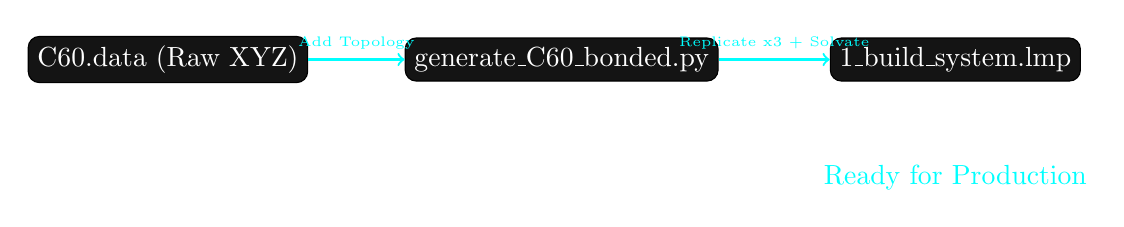
\begin{tikzpicture}[node distance=3cm, auto]
            \node [draw, rectangle, rounded corners, fill=codebg, text=white] (A) {C60.data (Raw XYZ)};
            \node [draw, rectangle, rounded corners, fill=codebg, text=white, right of=A, node distance=5cm] (B) {generate\_C60\_bonded.py};
            \node [draw, rectangle, rounded corners, fill=codebg, text=white, right of=B, node distance=5cm] (C) {1\_build\_system.lmp};
            
            \draw[->, thick, accentcyan] (A) -- node[above]{\tiny Add Topology} (B);
            \draw[->, thick, accentcyan] (B) -- node[above]{\tiny Replicate x3 + Solvate} (C);
            
            \node [below of=C, node distance=1.5cm, text=accentcyan] {Ready for Production};
        \end{tikzpicture}
    \end{center}

    \vspace{0.5cm}
    \textbf{Outcome:} A fully solvated, charge-neutral, topologically valid system prepared for GPU-accelerated equilibration.
\end{frame}
% =====================================================================
% SECTION: Main Simulation Protocol
% =====================================================================
\section{Main Simulation: Equilibration \& Production}

\begin{frame}
    \centering
    \Huge \textbf{The Main MD Script} \\
    \vspace{0.5cm}
    \Large Script: \texttt{2\_equilibrium\_version\_2\_w\_minimization.lmp} \\
    \vspace{1cm}
    \normalsize Solving the "Gas Phase Explosion" via Hybrid Hardware \& Numerical Stabilization
\end{frame}

% --- Slide: Hybrid Hardware Setup ---
\begin{frame}[fragile]{Initialization: Hybrid CPU/GPU Strategy}
    \textbf{The Hardware Bottleneck:}
    Standard \texttt{pppm/gpu} is fast but unstable during high-energy overlaps. \texttt{pppm/tip4p} (CPU) is stable but slow.
    
    \begin{lstlisting}[language=bash]
    units real
    atom_style full
    # GPU Acceleration for Force Calculation
    package gpu 1
    pair_style lj/cut/tip4p/long/gpu 2 3 2 1 0.1546 12.0
    \end{lstlisting}

    \textbf{Strategy:}
    \begin{enumerate}
        \item \textbf{Short Range Forces (LJ):} Offloaded to GPU ($O(N)$ neighbors).
        \item \textbf{Long Range Coulomb:} 
        \begin{itemize}
            \item During Minimization: CPU (Stability).
            \item During MD: GPU (Speed).
        \end{itemize}
    \end{enumerate}
\end{frame}
% =====================================================================
% SECTION: Initialization & Force Field Setup
% =====================================================================
\section{Script 2: Initialization \& Physics Setup}

% --- Slide: Base Units & Geometry ---
\begin{frame}[fragile]{1. Initialization \& Boundary Conditions}
    \begin{lstlisting}[language=bash]
    units real
    atom_style full
    boundary p p p
    atom_modify map array
    \end{lstlisting}

    \textbf{Physical Interpretations:}
    \begin{itemize}
        \item \texttt{units real}:
        \begin{itemize}
            \item Energy: kcal/mol
            \item Distance: \AA ngstroms ($10^{-10}$ m)
            \item Time: femtoseconds ($10^{-15}$ s)
        \end{itemize}
        \item \texttt{atom\_style full}: Required for \textbf{TIP4P water}. We need:
        \[ \{ID, MolID, Type, q, x, y, z\} \]
        Standard `atomic` style lacks Charge ($q$) and Molecule ID.
        \item \texttt{boundary p p p}: Periodic Boundary Conditions (PBC).
        \begin{equation}
            \mathbf{r}_{ij} = \min(|\mathbf{r}_i - \mathbf{r}_j + \mathbf{n}L|) \quad \mathbf{n} \in \mathbb{Z}^3
        \end{equation}
        Simulates an infinite bulk fluid using a finite box.
    \end{itemize}
\end{frame}

% --- Slide: Communication ---
\begin{frame}[fragile]{2. Parallel Communication Safety}
    \begin{lstlisting}[language=bash]
    comm_modify cutoff 18.0
    \end{lstlisting}

    \textbf{Why modify the cutoff?}
    LAMMPS decomposes the domain into spatial chunks (processors). Atoms near boundaries are "Ghost Atoms".
    
    \textbf{The Constraint:}
    \begin{equation}
        R_{comm} \ge R_{cut} + R_{skin}
    \end{equation}
    \begin{itemize}
        \item $R_{cut}$ (Coulomb) = 12.0 \AA.
        \item $R_{skin}$ (Neighbor) = 2.0 \AA.
        \item Minimum Safety = 14.0 \AA.
    \end{itemize}
    \textbf{Why 18.0 \AA?} We anticipate large volume fluctuations during the pressure ramp (Gas $\to$ Liquid transition). If the box expands rapidly, atoms move far. 18.0 \AA\ prevents "Lost Atom" errors during the 169,000 atm spike scenarios.
\end{frame}

% --- Slide: GPU Force Field ---
\begin{frame}[fragile]{3. GPU-Accelerated Force Field}
    \begin{lstlisting}[language=bash]
    pair_style lj/cut/tip4p/long/gpu 2 3 2 1 0.1546 12.0
    \end{lstlisting}

    \textbf{The TIP4P/2005 Model:}
    \textit{Reference: Abascal, J. L., \& Vega, C. (2005). J. Chem. Phys, 123(23).}
    
    The \texttt{0.1546} parameter is the distance $d_{OM}$ of the massless charge site $M$.
    \begin{itemize}
        \item \texttt{/gpu}: Offloads the $O(N)$ Lennard-Jones loop to CUDA cores.
        \item \texttt{/long}: Signals that Coulombics are handled by KSpace (PPPM).
    \end{itemize}
    
    \textbf{Interaction Types:}
    \begin{itemize}
        \item Type 1: Carbon (C60)
        \item Type 2: Oxygen (Water) - Central LJ site
        \item Type 3: Hydrogen (Water) - Charge only
    \end{itemize}
\end{frame}

% --- Slide: KSpace (PPPM) Details ---
\begin{frame}[fragile]{4. Long-Range Solver (The Fix)}
    \begin{lstlisting}[language=bash]
    kspace_style pppm/gpu 1.0e-4
    kspace_modify mesh 50 50 50 order 5 force/disp/real 0.8
    \end{lstlisting}

    \textbf{Particle-Particle Particle-Mesh (PPPM):}
    A variant of Ewald Summation. Maps charges to a 3D grid to solve Poisson's equation via FFT.
    
    \textbf{Parameter Choices:}
    \begin{itemize}
        \item \textbf{Tolerance ($10^{-4}$):} Relative error in forces. Standard for liquid water.
        \item \textbf{Mesh 50 50 50:} Locked to prevent "grid jitter" artifacts.
        \[ \text{Spacing } \approx 40\text{\AA} / 50 = 0.8 \text{\AA} \quad (\text{Rule of thumb: } < 1.0 \text{\AA}) \]
        \item \textbf{Order 5:} B-spline interpolation order. Higher order = smoother forces, less energy drift, but higher communication cost. 5 is high-precision (standard is 3 or 4).
    \end{itemize}
\end{frame}

% --- Slide: Coefficients ---
\begin{frame}[fragile]{5. Pair Coefficients (The Science)}
    \begin{lstlisting}[language=bash]
    # Water (TIP4P/2005)
    pair_coeff 2 2 0.1852 3.1589  # O-O epsilon(kcal/mol) sigma(Ang)
    
    # Carbon (C60)
    pair_coeff 1 1 0.07 3.4       # C-C (Standard Aromatic)
    
    # Cross Interaction (The Study Variable)
    variable epsilon_co equal ${EPSILON_CO}
    pair_coeff 1 2 ${epsilon_co} 3.2
    \end{lstlisting}

    \textbf{Lorentz-Berthelot Mixing Rules (Implicit):}
    Usually $\sigma_{ij} = \frac{\sigma_i + \sigma_j}{2}$.
    Here, $\sigma_{CO} = \frac{3.4 + 3.1589}{2} \approx 3.28$. We use $3.2$ explicitly based on literature tuning for carbon nanotubes in water.
    
    \textbf{The Variable $\epsilon_{CO}$:}
    Controls the wetting angle.
    \begin{itemize}
        \item $\epsilon < 0.1$: Hydrophobic (dewetting).
        \item $\epsilon > 0.2$: Hydrophilic (wetting).
    \end{itemize}
\end{frame}

% --- Slide: Neighbor Lists ---
\begin{frame}[fragile]{6. Neighbor Lists \& Binning}
    \begin{lstlisting}[language=bash]
    neighbor 2.0 bin
    neigh_modify delay 5 every 1 check yes
    \end{lstlisting}

    \textbf{Verlet Lists:}
    To avoid $O(N^2)$ distance checks, we keep a list of atoms within $R_{cut} + R_{skin}$.
    \begin{equation}
        R_{list} = 12.0 + 2.0 = 14.0 \text{ \AA}
    \end{equation}
    
    \textbf{Why \texttt{bin}?}
    LAMMPS sorts atoms into spatial bins (cells) of size $\approx R_{list}/2$.
    \begin{itemize}
        \item List build becomes $O(N)$ instead of $O(N^2)$.
        \item Crucial for our system ($N \approx 6000$) to run efficiently.
    \end{itemize}
    
    \textbf{Update Frequency:}
    `check yes`: Only rebuild list if an atom moved $> R_{skin}/2$ (1.0 \AA).
    `delay 5`: Don't even check for the first 5 steps after a rebuild (optimization).
\end{frame}

% --- Slide: Timestep ---
\begin{frame}[fragile]{7. Timestep \& Integration}
    \begin{lstlisting}[language=bash]
    timestep 2.0
    \end{lstlisting}

    \textbf{Integration Stability:}
    The Velocity-Verlet algorithm error scales as $O(\delta t^2)$.
    
    \textbf{Why 2.0 fs? (Standard is 1.0 fs)}
    \begin{itemize}
        \item \textbf{Restriction:} The fastest motion in water is the O-H bond vibration ($\tau \approx 10$ fs). To resolve it, we need $\delta t \approx 1$ fs.
        \item \textbf{Solution:} We use \texttt{fix shake} to freeze O-H bonds.
        \item \textbf{Result:} The fastest remaining motion is bond angle bending / LJ collisions. This allows extending $\delta t \to 2.0$ fs safely.
        \item \textbf{Benefit:} The simulation runs \textbf{2x faster}.
    \end{itemize}
\end{frame}
% --- Slide: The Critical PPPM Fix ---
\begin{frame}[fragile]{Critical Fix \#1: The PPPM Grid Lock}
    \textbf{The Root Cause of Failure:}
    Previously, the simulation exploded ($P > 169,000$ atm).
    \textit{Reason:} The Particle-Particle Particle-Mesh (PPPM) solver auto-resized the FFT grid when the box volume fluctuated, causing a discontinuous jump in Potential Energy.

    \begin{lstlisting}[language=bash]
    kspace_style pppm/gpu 1.0e-4
    # FIX: Lock the grid dimensions
    kspace_modify mesh 50 50 50 order 5
    \end{lstlisting}

    \textbf{Mathematics of PPPM:}
    The electrostatic energy is split (Ewald Summation):
    \begin{equation}
        E = E_{real} + E_{reciprocal} + E_{self} + E_{surface}
    \end{equation}
    $E_{reciprocal}$ is solved via Fast Fourier Transform (FFT) on a mesh.
    \[ \text{Grid Spacing } \Delta x = \frac{L_x}{N_{grid}} \]
    If $N_{grid}$ changes discretely while $L_x$ is changing, $\Delta E \to \infty$. \\
    \textbf{Solution:} Force $N_{grid} = (50, 50, 50)$ constant.
\end{frame}

% --- Slide: Stage 0 - Minimization ---
\begin{frame}[fragile]{Stage 0: Gentle Minimization (CPU)}
    \begin{lstlisting}[language=bash]
    # Switch to CPU pair style for stability
    pair_style lj/cut/tip4p/long ... 
    minimize 0.0 10.0 10 100
    \end{lstlisting}

    \textbf{Mathematical Objective:}
    Find the local minimum of the Potential Energy Surface (PES).
    \begin{equation}
        \nabla U(\mathbf{r}_1, \dots, \mathbf{r}_N) = \mathbf{0}
    \end{equation}
    We use the Conjugate Gradient method. We are NOT solving equations of motion (time is frozen). We simply move atoms along the force vector:
    \begin{equation}
        \mathbf{r}_{new} = \mathbf{r}_{old} + \gamma \mathbf{F}
    \end{equation}
    \textit{Purpose:} Resolve "bad contacts" (overlaps) created during the build phase ($r < \sigma$) which would cause infinite forces $\mathbf{F} \to \infty$ in MD.
\end{frame}

% --- Slide: Stage 1 - NVT ---
\begin{frame}[fragile]{Stage 1: NVT Thermalization}
    \begin{lstlisting}[language=bash]
    timestep 2.0
    velocity all create 300.0 ... dist gaussian
    fix mynvt all nvt temp 300.0 300.0 100.0
    \end{lstlisting}

    \textbf{1. Timestep ($dt = 2.0$ fs):}
    Possible because SHAKE removes high-frequency O-H bond vibrations ($f \approx 10^{14}$ Hz). Speedup: $2\times$.

    \textbf{2. Velocity Initialization:}
    Assigns velocities from Maxwell-Boltzmann distribution:
    \begin{equation}
        P(v) = 4\pi \left( \frac{m}{2\pi k_B T} \right)^{3/2} v^2 \exp\left( \frac{-mv^2}{2k_B T} \right)
    \end{equation}

    \textbf{3. NVT Ensemble (Canonical):}
    Constant $N$ (atoms), $V$ (volume), $T$ (temp). The barostat is OFF. Pressure will be high ($\sim 800$ atm) because we packed atoms into a fixed box.
\end{frame}

\begin{frame}(Let's see the Temperature Equilibration)
    \begin{figure}
        \centering
        \includegraphics[width=0.7\textwidth]{../analysis/plots/01_temperature_evolution.png}
        % \caption{System after NVT Thermalization: C60 molecules (gray) surrounded by equilibrated water (red/white).}
    \end{figure}
\end{frame}

% =====================================================================
% SECTION: DETAILED PROTOCOL (Stage 1.5 to End)
% =====================================================================
\section{Protocol Deep Dive: Stage 1.5 to Production}

% --- Slide: Stage 1.5 Concept ---
\begin{frame}[fragile]{Stage 1.5: Pre-Equilibration (The Pressure Bridge)}
    \textbf{The Logic:} 
    In the failed run, NVT (Fixed V) $\to$ NPT (1 atm) caused a shock.
    \textit{Physics:} Water has a high Bulk Modulus ($K \approx 2.2$ GPa). A tiny density mismatch results in massive pressure ($P \approx 10^5$ atm).
    
    \begin{lstlisting}[language=bash]
    # Fix #2: Target 100 atm, High Damping
    fix mynpt_pre all npt temp 300 300 100 iso 100 100 5000
    \end{lstlisting}

    \textbf{Parameter breakdown:}
    \begin{itemize}
        \item \texttt{iso 100 100}: We target an intermediate pressure. This allows the box to expand, but effectively "pushes back" to prevent the water from flashing into gas.
        \item \texttt{Pdamp 5000}: The barostat relaxation time $\tau_P$.
        \begin{equation}
            \dot{V} \propto \frac{1}{\tau_P} (P_{inst} - P_{target})
        \end{equation}
        A large $\tau_P$ (5000 fs) makes the box volume react \textit{slowly}, preventing explosive expansion.
    \end{itemize}
\end{frame}

% --- Slide: Stage 2 Ramp ---
\begin{frame}[fragile]{Stage 2: The Pressure Ramp (Fix \#3)}
    \textbf{The Command:}
    \begin{lstlisting}[language=bash]
    fix mynpt_ramp all npt ... iso 100.0 1.0 2000.0 drag 2.0
    \end{lstlisting}
    
    \textbf{What is happening?}
    We linearly interpolate the target pressure $P_{ext}(t)$ from 100 atm to 1 atm over 50,000 steps.

    \textbf{Mathematics of `drag 2.0`:}
    The volume equation of motion in the Nosé-Hoover-Andersen barostat includes a fictitious "piston mass" $W$. The `drag` adds a friction term $\Gamma$:
    \begin{equation}
        W \ddot{V} = V(P_{int} - P_{ext}) - \underbrace{\Gamma \dot{V}}_{\text{Drag Force}}
    \end{equation}
    \textit{Why?} Without drag, the box volume $V(t)$ oscillates like a harmonic oscillator (ringing) after a pressure drop. The drag term acts as a critical damper ($\zeta \approx 1$), stabilizing the density smoothy.
\end{frame}

% --- Slide: Stage 3 Strategy ---
\begin{frame}[fragile]{Stage 3: Two-Phase NPT Equilibration}
    We do not simply "turn on" NPT. We use a refined 2-phase approach.
    
    \textbf{Phase 1: Stabilization (400 ps)}
    \begin{lstlisting}[language=bash]
    fix mynpt_gentle all npt/gpu ... iso 1.0 1.0 5000.0
    \end{lstlisting}
    \textit{Action:} Uses \texttt{npt/gpu} (offloads virial calc to GPU). Keeps $\tau_P = 5000$ fs. The system gently settles into the 1 atm basin.

    \textbf{Phase 2: Convergence (600 ps)}
    \begin{lstlisting}[language=bash]
    fix mynpt_standard all npt/gpu ... iso 1.0 1.0 2000.0
    \end{lstlisting}
    \textit{Action:} We tighten $\tau_P$ to 2000 fs. This allows standard thermal fluctuations of the volume, necessary for correct density sampling.
\end{frame}

% --- Slide: Density Checkpoints ---
\begin{frame}[fragile]{Safety Mechanism: Density Checkpoints}
    Simulations can fail silently. We added logic gates to the script.

    \begin{lstlisting}[language=bash]
    variable current_dens equal density
    if "${current_dens} < 0.85 || ${current_dens} > 1.15" then &
       "print 'ERROR: Density outside expected range'" &
       "quit 1"
    \end{lstlisting}

    \textbf{The Gas Phase Detection:}
    In your previous failed run, $\rho \to 0.025$ g/cm$^3$.
    This check catches that failure \textit{before} wasting 4 nanoseconds of GPU time on a gas-phase simulation.
\end{frame}

% --- Slide: Stage 4 Production (MTK) ---
\begin{frame}[fragile]{Stage 4: Production - The MTK Correction}
    \begin{lstlisting}[language=bash]
    fix mynpt all npt/gpu temp 300 300 100 iso 1 1 1000 mtk yes
    \end{lstlisting}

    \textbf{Detailed Math: Martyna-Tobias-Klein (MTK):}
    Standard Nosé-Hoover generates the NPT distribution only in the thermodynamic limit ($N \to \infty$). For finite systems, it misses a metric factor in phase space.
    
    MTK adds a correction to the Hamiltonian equations:
    \begin{equation}
        \dot{\mathbf{p}}_i = \mathbf{F}_i - \frac{\mathbf{p}_i \pi_{\epsilon}}{Q} - \underbrace{\frac{d-1}{dN k_B T} \epsilon \mathbf{p}_i}_{\text{MTK Term}}
    \end{equation}
    \textit{Significance:} Ensures that the fluctuations in Volume $\langle (\delta V)^2 \rangle$ (related to compressibility) are statistically rigorous.
\end{frame}

% --- Slide: Analysis - RDF Correction ---
\begin{frame}[fragile]{Analysis: C60-C60 RDF Issue (Sadly I identified it a few hours ago)}
    \textbf{The Problem:} 
    C60 molecules have IDs 1, 2, 3. But they contain 180 atoms total.
    Standard RDF counts distances between \textit{all} pairs of type 1 (Carbon).
    \[ \text{Intra-molecular C-C bonds: } 1.4 \text{\AA} \quad (\text{Noise}) \]
    \[ \text{Inter-molecular C-C gap: } 10-20 \text{\AA} \quad (\text{Signal}) \]

    \textbf{The Fix:}
    \begin{lstlisting}[language=bash]
    neigh_modify exclude molecule/intra carbon
    compute rdf_CC all rdf 150 1 1
    neigh_modify exclude none  # Restore immediately
    \end{lstlisting}
    
    \textbf{Set Theory:}
    Let $D = \{ ||\mathbf{r}_i - \mathbf{r}_j|| \}$.
    We compute $D_{inter} = D \setminus \{ \text{pairs where } mol(i) == mol(j) \}$.
\end{frame}

% --- Slide: Analysis - Outputs ---
\begin{frame}[fragile]{Analysis: Observables \& MSD}
    \textbf{1. Mean Squared Displacement (MSD):}
    \begin{lstlisting}[language=bash]
    compute msd_water oxygen msd
    \end{lstlisting}
    Used to calculate Self-Diffusion Coefficient ($D_{water}$):
    \begin{equation}
        D_{water} = \lim_{t \to \infty} \frac{1}{6t} \langle |\mathbf{r}(t) - \mathbf{r}(0)|^2 \rangle
    \end{equation}
    \textit{Goal:} See if hydrophobic C60 speeds up water diffusion vs hydrophilic.

    \textbf{2. High-Res Thermodynamics:}
    \begin{lstlisting}[language=bash]
    fix thermo_detailed all ave/time 10 10 100 ...
    \end{lstlisting}
    Samples every 0.2 ps. Used to compute heat capacity ($C_p$) and compressibility ($\kappa_T$) via fluctuation formulas:
    \begin{equation}
        \langle \delta H^2 \rangle = k_B T^2 C_p
    \end{equation}
\end{frame}

% =========================
% SECTION: RESULTS (Plots per Module)
% =========================
\section{Results: Module Outputs}

% -- Module 1: Thermodynamic Analysis (formulas + plots)
\begin{frame}{Module 01: Thermodynamic Analysis - Math}
    	extbf{Ensemble averages \& fluctuations}
    \begin{itemize}
        \item Ensemble average: $\langle X \rangle = \frac{1}{N} \sum_{i=1}^N X_i$
        \item Fluctuations: $\sigma_X = \sqrt{\langle X^2 \rangle - \langle X \rangle^2}$
        \item Equilibration detection: linear drift $X(t)=\alpha t + \beta$, equilibrium when $\alpha\approx 0$.
        \item Autocorrelation: $C_X(\tau)=\frac{\langle (X(t)-\langle X\rangle)(X(t+\tau)-\langle X\rangle)\rangle}{\sigma_X^2}$
    \end{itemize}
\end{frame}

\begin{frame}{01 Temperature Evolution}
    \begin{center}
        \includegraphics[width=0.85\textwidth]{../analysis/plots/01_temperature_evolution.png}
    \end{center}
\end{frame}

\begin{frame}{02 Pressure Analysis}
    \begin{center}
        \includegraphics[width=0.85\textwidth]{../analysis/plots/02_pressure_analysis.png}
    \end{center}
\end{frame}

\begin{frame}{03 Density Analysis}
    \begin{center}
        \includegraphics[width=0.85\textwidth]{../analysis/plots/03_density_analysis.png}
    \end{center}
\end{frame}

\begin{frame}{04 Energy Analysis}
    \begin{center}
        \includegraphics[width=0.85\textwidth]{../analysis/plots/04_energy_analysis.png}
    \end{center}
\end{frame}

\begin{frame}{05 Comparison Matrix}
    \begin{center}
        \includegraphics[width=0.85\textwidth]{../analysis/plots/05_comparison_matrix.png}
    \end{center}
\end{frame}

% -- Module 2: Equilibration Stability
\begin{frame}{Module 02: Equilibration Stability - Math}
    \begin{itemize}
        \item Block averaging: divide trajectory into $M$ blocks, check variance scaling $\sigma_B^2\propto 1/B$.
        \item Autocorrelation time and effective sample size via FFT (Wiener-Khinchin).
    \end{itemize}
\end{frame}

\begin{frame}{06 Autocorrelation Analysis}
    \begin{center}
        \includegraphics[width=0.85\textwidth]{../analysis/plots/06_autocorrelation_analysis.png}
    \end{center}
\end{frame}

\begin{frame}{07 Block Averaging}
    \begin{center}
        \includegraphics[width=0.85\textwidth]{../analysis/plots/07_block_averaging.png}
    \end{center}
\end{frame}

\begin{frame}{08 Running Averages}
    \begin{center}
        \includegraphics[width=0.85\textwidth]{../analysis/plots/08_running_averages.png}
    \end{center}
\end{frame}

\begin{frame}{09 Stability Metrics}
    \begin{center}
        \includegraphics[width=0.85\textwidth]{../analysis/plots/09_stability_metrics.png}
    \end{center}
\end{frame}

% -- Module 3: RDF Structural Analysis
\begin{frame}{Module 03: RDF - Math}
    \begin{itemize}
        \item Radial distribution: $g(r)=\frac{1}{4\pi r^2 \rho N} \sum_{i}\sum_{j\ne i}\delta(r-r_{ij})$.
        \item Coordination number: $N(r_{cut})=4\pi\rho\int_0^{r_{cut}} r^2 g(r) \, dr$.
    \end{itemize}
\end{frame}

\begin{frame}{10 RDF Comparison}
    \begin{center}
        \includegraphics[width=0.85\textwidth]{../analysis/plots/10_rdf_comparison.png}
    \end{center}
\end{frame}

\begin{frame}{11 C-O RDF Detailed}
    \begin{center}
        \includegraphics[width=0.85\textwidth]{../analysis/plots/11_co_rdf_detailed.png}
    \end{center}
\end{frame}

\begin{frame}{12 Coordination Numbers}
    \begin{center}
        \includegraphics[width=0.85\textwidth]{../analysis/plots/12_coordination_numbers.png}
    \end{center}
\end{frame}

% -- Module 4/5: Water Structure / Plotting
\begin{frame}{Module 05: Water Structure - Math}
    \begin{itemize}
        \item Tetrahedral order: $q=1-\tfrac{3}{8}\sum_{j=1}^3\sum_{k=j+1}^4\left(\cos\psi_{jk}+\tfrac{1}{3}\right)^2$.
        \item Hydrogen bond criteria: $r_{OO}<3.5\\AA$, $\angle H-O...O < 30^\circ$.
    \end{itemize}
\end{frame}

\begin{frame}{13 Tetrahedral Order}
    \begin{center}
        \includegraphics[width=0.85\textwidth]{../analysis/plots/13_tetrahedral_order_analysis.png}
    \end{center}
\end{frame}

\begin{frame}{14 Steinhardt Order Parameters}
    \begin{center}
        \includegraphics[width=0.85\textwidth]{../analysis/plots/14_steinhardt_order_parameters.png}
    \end{center}
\end{frame}

\begin{frame}{15 Shape Parameters (Asphericity)}
    \begin{center}
        \includegraphics[width=0.85\textwidth]{../analysis/plots/15_shape_parameters_oblate_prolate.png}
    \end{center}
\end{frame}

\begin{frame}{16 Coordination \& H-bond Analysis}
    \begin{center}
        \includegraphics[width=0.85\textwidth]{../analysis/plots/16_coordination_hbond_analysis.png}
    \end{center}
\end{frame}

\begin{frame}{17 MSD / Diffusion Analysis}
    \begin{center}
        \includegraphics[width=0.85\textwidth]{../analysis/plots/17_msd_diffusion_analysis.png}
    \end{center}
\end{frame}

% -- Module 6: MSD Validation
\begin{frame}{Module 06: MSD - Math}
    	extbf{MSD: } $\\mathrm{MSD}(t)=\\langle |\\mathbf{r}(t)-\\mathbf{r}(0)|^2\\rangle$. \\
    Diffusion: $D=\\lim_{t\\to\\infty}\\mathrm{MSD}(t)/(6t)$.
\end{frame}

\begin{frame}{18 MSD Evolution}
    \begin{center}
        \includegraphics[width=0.85\\textwidth]{../analysis/plots/18_msd_evolution.png}
    \end{center}
\end{frame}

% -- Module 7: High Priority Additional Analysis
\begin{frame}{Module 07: High-Priority Analysis - Math}
    \begin{itemize}
        \item Inter-fullerene distance time-series and aggregation metrics.
        \item Thermodynamic response functions via fluctuations: $C_V=\\langle \\delta E^2\\rangle/(k_B T^2)$, $\\kappa_T=\\langle \\delta V^2\\rangle/(k_B T \\langle V\\rangle)$.
    \end{itemize}
\end{frame}

\begin{frame}{19 C60 Distance Time Series}
    \begin{center}
        \includegraphics[width=0.85\\textwidth]{../analysis/plots/19_c60_distance_timeseries.png}
    \end{center}
\end{frame}

\begin{frame}{20 Aggregation Analysis}
    \begin{center}
        \includegraphics[width=0.85\\textwidth]{../analysis/plots/20_c60_aggregation_analysis.png}
    \end{center}
\end{frame}

\begin{frame}{21 C60 Diffusion}
    \begin{center}
        \includegraphics[width=0.85\\textwidth]{../analysis/plots/21_c60_diffusion.png}
    \end{center}
\end{frame}

\begin{frame}{22 Thermodynamic Response Functions}
    \begin{center}
        \includegraphics[width=0.85\\textwidth]{../analysis/plots/22_thermodynamic_response_functions.png}
    \end{center}
\end{frame}

% -- Module 8: PPM Snapshot Analysis
\begin{frame}{Module 08: PPM Snapshot Analysis - Math}
    \begin{itemize}
        \item Brightness: mean pixel intensity $\\mu_I$; Contrast: $\\sigma_I$ (std dev).
    \end{itemize}
\end{frame}

\begin{frame}{23 PPM Snapshot Montage}
    \begin{center}
        \includegraphics[width=0.85\\textwidth]{../analysis/plots/23_ppm_snapshot_montage.png}
    \end{center}
\end{frame}

\begin{frame}{24 PPM Metrics}
    \begin{center}
        \includegraphics[width=0.85\\textwidth]{../analysis/plots/24_ppm_metrics.png}
    \end{center}
\end{frame}

% -- Module 9: Equilibration Pathway
\begin{frame}{Module 09: Equilibration Pathway - Math}
    	extbf{Stages:} NVT Thermalization, Pre-equilibration, Pressure ramp, NPT equilibration.\\
    Use multi-panel evolution plots to show stage-wise convergence.
\end{frame}

\begin{frame}{25 Equilibration Pathway}
    \begin{center}
        \includegraphics[width=0.85\\textwidth]{../analysis/plots/25_equilibration_pathway.png}
    \end{center}
\end{frame}

% -- Module 10: Structural Data Analysis
\begin{frame}{Module 10: Structural Data - Math}
    \begin{itemize}
        \item Bond length distributions, hydration shell counts (e.g. $r_{C-O}<r_{shell}$).
        \item Displacement vectors $\\Delta \\mathbf{r}=\\mathbf{r}_{final}-\\mathbf{r}_{initial}$.
    \end{itemize}
\end{frame}

\begin{frame}{26 Bond Lengths}
    \begin{center}
        \includegraphics[width=0.85\\textwidth]{../analysis/plots/26_bond_lengths.png}
    \end{center}
\end{frame}

\begin{frame}{27 Hydration Shell}
    \begin{center}
        \includegraphics[width=0.85\\textwidth]{../analysis/plots/27_hydration_shell.png}
    \end{center}
\end{frame}

\begin{frame}{28 Radial Distributions (static)}
    \begin{center}
        \includegraphics[width=0.85\\textwidth]{../analysis/plots/28_radial_distributions.png}
    \end{center}
\end{frame}

% Finalize document
\end{document}
